% Created 2022-07-15 Fri 09:57
% Intended LaTeX compiler: xelatex
\documentclass[8pt,twoside,landscape]{extarticle}
\usepackage{graphicx}
\usepackage{longtable}
\usepackage{wrapfig}
\usepackage{rotating}
\usepackage[normalem]{ulem}
\usepackage{amsmath}
\usepackage{amssymb}
\usepackage{capt-of}
\usepackage{hyperref}
\usepackage{subcaption}
\usepackage[newfloat]{minted}
\usepackage{color}
\usepackage{listings}
\usepackage[top=5mm,bottom=5mm,right=5mm,left=5mm,landscape]{geometry}
\usepackage{multicol}
\usepackage{enumitem}
\usepackage{fancyhdr}
\usepackage{caption}
\usepackage{algorithm}
\usepackage{algpseudocode}
\usepackage{float}
\setlist{noitemsep, topsep=0pt}
\setlength{\parindent}{0pt}
\setlength{\columnseprule}{0.2pt}
\definecolor{mygreen}{rgb}{0,0.6,0}
\definecolor{mygray}{rgb}{0.5,0.5,0.5}
\definecolor{mymauve}{rgb}{0.58,0,0.82}
\lstset{ backgroundcolor=\color{white}, basicstyle=\footnotesize, breaklines=true, captionpos=b, commentstyle=\color{mygreen}, escapeinside={\%*}{*)},keywordstyle=\color{blue}, stringstyle=\color{mymauve},}
\author{Olivier Lischer}
\date{\today}
\title{ParProg Summary}
\hypersetup{
 pdfauthor={Olivier Lischer},
 pdftitle={ParProg Summary},
 pdfkeywords={},
 pdfsubject={},
 pdfcreator={Emacs 27.2 (Org mode 9.5.3)}, 
 pdflang={English}}
\begin{document}

\begin{multicols}{5}

\section{Multi-Threading Basics}
\label{sec:orgf797b2f}
\subparagraph{Cooperative Multi-Tasking} \
\label{sec:orgf851e48}
In this model the thread works as long as it wants.
If the thread want to wait, it must initiate the process by itself.
A scheduler can not interrupt a running thread!

\subparagraph{Preemptive Multi-Tasking} \
\label{sec:orgdba0338}

The scheduler uses a \emph{Timer Interrupt} to interrupt a running thread.
Each Thread can work for a specific max. interval.
After that interval is over and the thread is not finished, the thread is interrupted and is added to the \emph{Ready-Queue}.


\subparagraph{Thread States} \
\label{sec:org67b074d}

{
\begin{center}
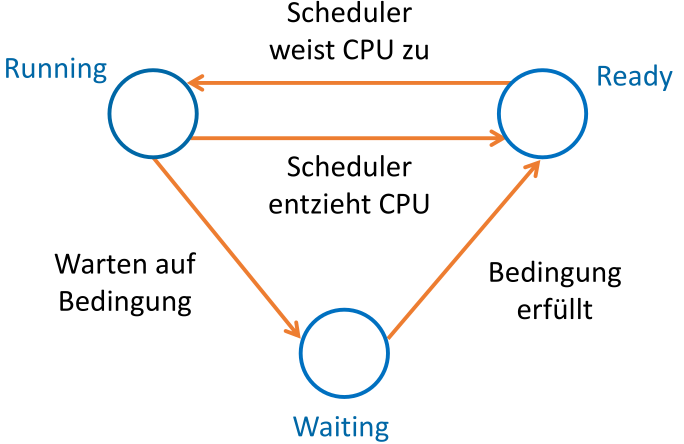
\includegraphics[width=.9\linewidth]{img/thread_states.png}
\end{center}
\captionof{figure}{Thread States}\label{fig:thread-states}
}
\subparagraph{JVM termination} \
\label{sec:org1526c34}
The JVM runs as long as at least one non-daemon thread is running.
If the last non-daemon thread is terminated then the JVM is shutdown and all daemon threads are killed uncontrolled.
Therefore, it is not possible to implement something like goodbye message when the thread terminates.
If inside a thread an uncaught exception occurs the other threads are \textbf{not} terminated and keep working.
\section{Monitor}
\label{sec:org584c3ae}
\subparagraph{Monitor} \
\label{sec:org4a9e73c}
The monitor is a synchronisation mechanism which use the \emph{Wait \& Signal} / \emph{Signal \& Continue} mechanism.
\begin{enumerate}
\item Fight for lock
\begin{itemize}
\item winner: enters the monitor (acquire the lock)
\item others: wait for entrance
\end{itemize}
\item Thread in monitor does work
\begin{itemize}
\item if done: leaves monitor and wakes up other threads (\texttt{notify()} / \texttt{notifyAll()})
\item condition not satisfied: leaves monitor and goes to the right and wake up other threads (Wait on signal)
\end{itemize}
\item Go to 1.
\end{enumerate}

{
\begin{center}
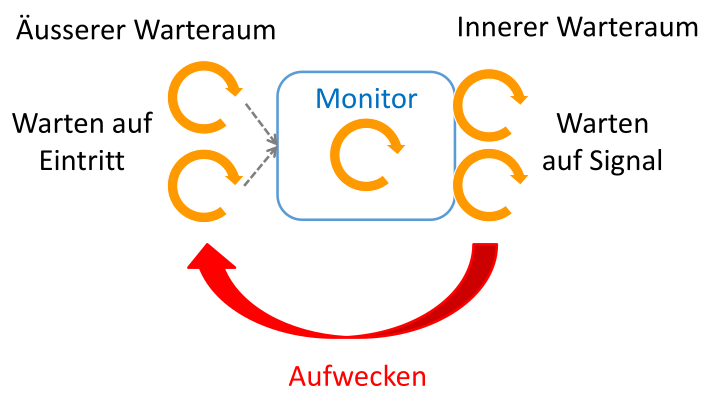
\includegraphics[width=.9\linewidth]{img/monitor.png}
\end{center}
\captionof{figure}{A monitor}\label{fig:monitor}
}
\subparagraph{Single Notify} \
\label{sec:org0bb8f11}
A single notify can only be used when:
\begin{enumerate}
\item every thread has the same condition
\item only one \textbf{single} thread can make progress (One-In/One-Out)
\end{enumerate}
\subparagraph{Thread Wake up} \
\label{sec:orge503457}
\begin{enumerate}
\item notifyAll(), notify()
\item InterruptedException
\item Spurious Wake up (falsely wake up POSIX Thread API)
\end{enumerate}
\section{Synchronization Mechanism}
\label{sec:org2f3b625}
\subparagraph{Semaphore} \
\label{sec:org4b5704f}
\lstset{language=java,label= ,caption= ,captionpos=b,numbers=none}
\begin{lstlisting}
public class BoundedBufferSemaphore<T> {
    private Queue<T> queue = new LinkedList<>();

    public BoundedBufferSemaphore(int capacity) {
	upperLimit = new Semaphore(capacity, true);
    }

    public void put(T element) throws InterruptedException {
	upperLimit.acquire(); // counter--
	mutex.acquire(); queue.add(element); mutex.release();
	lowerLimit.release(); //counter++
    }
}
\end{lstlisting}
\subparagraph{Lock \& Conditions} \
\label{sec:org34e6cab}
{
\begin{center}
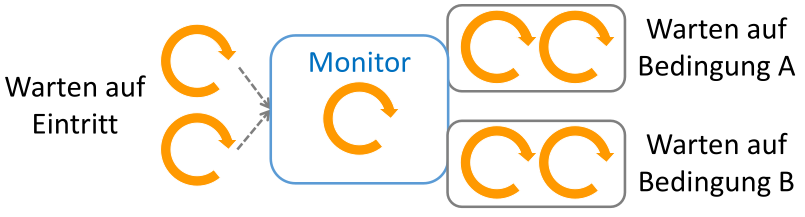
\includegraphics[width=.9\linewidth]{img/lock_and_conditions.png}
\end{center}
\captionof{figure}{Lock & Conditions}\label{fig:lock-and-conditions}
}

\lstset{language=java,label= ,caption= ,captionpos=b,numbers=none}
\begin{lstlisting}
public class WarehouseWithLockCondition {
    public WarehouseWithLockCondition(int capacity, boolean fair) {
	lock = new ReentrantLock(fair);
	nonEmpty = lock.newCondition();
	nonFull = lock.newCondition();
    }
    @Override
    public void put(int amount) throws InterruptedException {
	lock.lock();
	try {
	    nonFull.await();
	    nonEmpty.signalAll();
	} finally { lock.unlock(); }
    }
}
\end{lstlisting}

\subparagraph{Read-Write Locks} \
\label{sec:org08f1a11}
\lstset{language=java,label= ,caption= ,captionpos=b,numbers=none}
\begin{lstlisting}
var rwLock = new ReentrantReadWriteLock(true);
rwLock.readLock().lock();
// read-only accesses
rwLock.readLock().unlock();
rwLock.writeLock().lock();
// write (and read) accesses
rwLock.writeLock().unlock();
\end{lstlisting}
\subparagraph{CountdownLatch} \
\label{sec:org555875b}
\lstset{language=java,label= ,caption= ,captionpos=b,numbers=none}
\begin{lstlisting}
CountDownLatch waitForAll = new CountDownLatch(this.CARS);
protected void test() throws InterruptedException {
    waitForAll.countDown();
    waitForAll.await();
}
\end{lstlisting}
\subparagraph{Cyclic Barrier} \
\label{sec:orgdba2818}
\lstset{language=java,label= ,caption= ,captionpos=b,numbers=none}
\begin{lstlisting}
var gameRound = new CyclicBarrier(5);
/* 5 different players / threads */
while (true) gameRound.await();
\end{lstlisting}

\subparagraph{Rendez-Vous} \
\label{sec:orgba944c4}
\begin{itemize}
\item Without exchange: \texttt{new CyclicBarrier(2);}
\item With exchange: \texttt{Exchanger.exchange(something)};
\end{itemize}
\subparagraph{Monitor in .NET} \
\label{sec:org6acfe89}
\lstset{language=csharp,label= ,caption= ,captionpos=b,numbers=none}
\begin{lstlisting}
class BankAccount {
    private decimal balance;
    private object syncObject = new();
    public void Deposite(decimal amount) {
	lock (syncObject) {
	    balance += amaount;
	    Monitor.PulseAll(syncObject);
	    //Monitor.Wait(syncObject);
	}
    }
}
\end{lstlisting}
\section{Threats}
\label{sec:org2a7dfa4}
\subparagraph{General} \
\label{sec:orgb207efb}
Race Condition, Deadlock, Starvation
\subparagraph{Confinement} \
\label{sec:org66bc4ae}
Under confinement, we understand a structure that guaranties that only one thread can access an object at time.
\begin{itemize}
\item \emph{Thread Confinement}: an object belongs to a single thread and is used only be this thread
\item \emph{Object Confinement}: an object is encapsulated in an already synchronized object
\end{itemize}

{
\begin{center}
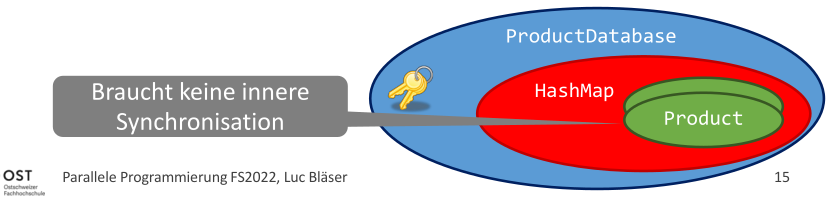
\includegraphics[width=.9\linewidth]{img/object_confinement.png}
\end{center}
\captionof{figure}{Example of object confinement}\label{fig:example-of-object-confinement}
}
\section{Thread Pool}
\label{sec:org9115dc9}
\subparagraph{Thread Pool} \
\label{sec:org86d8aae}
A thread pool consists of a task queue and n worker threads.
A new task is inserted in the queue.
The new free thread from the thread pool takes the first task from the queue and process it.

\subparagraph{Work stealing} \
\label{sec:org770b5fe}
Each Worker Thread has also its own task queue.
A worker thread takes some task from the global queue and move it to the local queue.
If the another worker thread wants to work but the global queue is empty, it steals it from other worker threads.
\subparagraph{Thread Injection} \
\label{sec:org518f25c}
When I injection new Threads in the thread pool during runtime is called \emph{Thread Injection}.
This can mitigate possible deadlocks when two task are not indepentend (only if not max threads is set).
\subparagraph{Number of Threads} \
\label{sec:orgdc34d9d}
A thread pool has as much threads as processors (cores) and little bit more.
A little bit more than the number of processors is ideally because when one thread has to wait for I/O another thread can use the processor:

\subparagraph{ForkJoinPool} \
\label{sec:org89729dc}
\lstset{language=java,label= ,caption= ,captionpos=b,numbers=none}
\begin{lstlisting}
var threadPool = new ForkJoinPool();
Future<Integer> future = threadPool.submit(() -> {
	int value = 1;
	return value;
});
Integer i = future.get();

class MyTask extends RecursiveTask<Integer> {
    boolean finished = false;
    @Override
    protected Integer compute() {
	if (finished) return 1;
	var left = new MyTask();
	var right = new MyTask();
	left.fork();
	right.fork();
	return left.join() + right.join();
    }
}
var n = threadPool.invoke(new MyTask());
\end{lstlisting}
\subparagraph{.NET} \
\label{sec:org4568f30}
\lstset{language=csharp,label= ,caption= ,captionpos=b,numbers=none}
\begin{lstlisting}
Task task1 = Task.Run(() => { /* Do some stuff */ });
task1.Wait(); // blocking

// Task with return value
Task task2 = Task.Run(() => { return 3;});
Console.Write(task.Result); // blocking

// Task with Sub Tasks
Task.Run(() => {
    var left = Task.Run(() => Count(leftPart));
    var right = Task.Run(() => Count(rightPart));
    int result = left.Result + right.Result;
    return result;
});

// Parallele Statements
Parallel.Invoke(
    () => MergeSort(l, m),
    () => MergeSort(m, r)
);

// Parallel Loop
Parallel.ForEach(list, file => Convert(file));

// Parallel For - only if iterations are indepentend
Parallel.For(0, array.Length, i => DoComputation(array[i]));
\end{lstlisting}
\section{Async}
\label{sec:orgbcade66}
\subparagraph{Types} \
\label{sec:org838d9ea}
You differ between two types of asynchrony:
\begin{itemize}
\item caller centric (pull)
\begin{itemize}
\item The caller waits for task end and pulls the result
\end{itemize}
\item callee centric (push)
\begin{itemize}
\item task forwards the result to the successor task
\end{itemize}
\end{itemize}
\subparagraph{Continuation C\#} \
\label{sec:org715eddd}
Exception in Fire \& Forget are ignored.
To handle exception you have to wait synchrony for finishing the task.

\lstset{language=csharp,label= ,caption= ,captionpos=b,numbers=none}
\begin{lstlisting}
Task.Run(task1).
    ContinueWith(task2).
    ContinueWith(task3).Wait();
Task.WhenAll(task1, task2).
    ContinueWith(continuation).Wait();
Task.WhenAny(task1, task2).
    ContinueWith(continuation).Wait();
\end{lstlisting}
\subparagraph{CompleatableFuture Java} \
\label{sec:orgc31794f}
\lstset{language=java,label= ,caption= ,captionpos=b,numbers=none}
\begin{lstlisting}
var all = CompletableFuture.<Void>completedFuture(null);
for (int i = 0; i < LINKS.length; i++) {
    var link = LINKS[i];
    var future = downloader.asyncDownloadUrl(link).thenAcceptAsync(result -> { /*Stuff*/ });
    all = CompletableFuture.allOf(all, future);
}
all.thenAcceptAsync(voids -> { /*Stuff*/ }).join();
\end{lstlisting}
\section{Memory Modell}
\label{sec:org943df64}
\subparagraph{Atomicity} \
\label{sec:org26e810d}
Single reads / writes are atomic for:
\begin{itemize}
\item primitive data types until 32 bits
\item object references
\item long and double only with the \texttt{volatile} keyword (only Java)
\end{itemize}
Java: \texttt{AtomicBoolean} / C\# \texttt{Interlocked}

\subparagraph{Visibility} \
\label{sec:org5a36b6e}
Java guaranties the following visibility:
\begin{itemize}
\item changes before release are visible at acquire
\item changes until write are visible at read
\item the thread sees the correct start values and Join the output of the thread
\item initialization of final variables (only relevant if you get the object from a data race!)
\end{itemize}

\subparagraph{Ordering} \
\label{sec:orgd5d273e}
The order of the visibility is the same as in visibility.
Additional:
\begin{itemize}
\item synchronization instructions are never reordered to each other
\item Lock/Unlock, volatile, thread start / join are never reordered
\item if everything is a synchronization mechanism than we talk about total order
\end{itemize}

\subparagraph{Voltile} \
\label{sec:orge50d5dd}
The \texttt{volatile} keyword in .NET is only a Half Fence.
That means
\begin{itemize}
\item volatile writes: previous access stay before
\item volatile reads: following access remain after
\end{itemize}
In Java is a Full Fence (no reordering).
\lstset{language=csharp,label= ,caption= ,captionpos=b,numbers=none}
\begin{lstlisting}
Thread.MemoryBarrier(); // Full Fence
\end{lstlisting}
\section{GPU}
\label{sec:orgb5d2c1f}
\begin{description}
\item[{latency}] how long does it take to execute a single instruction / operation
\item[{throughput}] number of instructions / operations completed per second
\end{description}
\subparagraph{Arithmetic Intensity} \
\label{sec:orge42362b}

\begin{equation}
  \begin{align}
    &t_c > t_m \\
    &\frac{ops}{BW_c} > \frac{bytes}{BW_m} \\
    &\frac{ops}{bytes} > \frac{BW_C}{BW_m} \\
    &\text{Arithmetic intensity} = \frac{BW_c}{BW_m}
  \end{align}
\end{equation}

\subparagraph{Thermilogy} \
\label{sec:orgc616b64}
{
\begin{center}
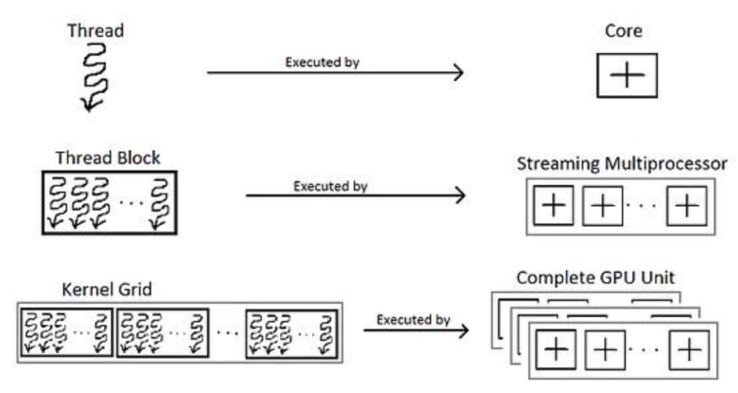
\includegraphics[width=.9\linewidth]{img/cuda_to_gpu_analogy.png}
\end{center}
\captionof{figure}{CUDA concepts on the GPU}\label{fig:cuda-concepts-on-the-gpu}
}

\subparagraph{Classification} \
\label{sec:orgf7cd578}

{
\begin{center}
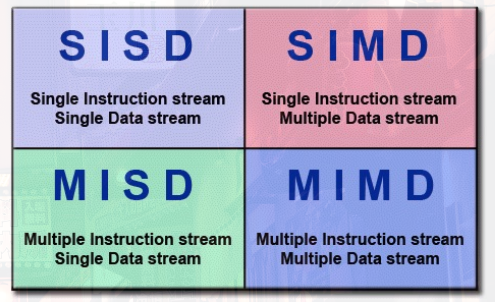
\includegraphics[width=.9\linewidth]{img/flynn_classical_taxonomy.png}
\end{center}
\captionof{figure}{Flynn's Classical Taxonomy}\label{fig:flynns-classical-taxonomy}
}

\subparagraph{Launch Kernel} \
\label{sec:orgb988624}
\lstset{language=C,label= ,caption= ,captionpos=b,numbers=none}
\begin{lstlisting}
__global__
void VectorAddKernel(float *a, float *b, float *c, int size) {
  int i = blockIdx.x * blockDim.x + threadIdx.x;
  if (i < size) {
    c[i] = a[i] + b[i];
  }
}
int blockSize = 1024;
int gridSize = (numElements + blockSize - 1) / blockSize;
VectorAddKernel<<<gridSize, blockSize>>>(d_a, d_b, d_c, numElements);
\end{lstlisting}
\subparagraph{Thread Hierarchy} \
\label{sec:org8a807c7}
A Kernel is executed in a single thread.
The single thread is executed simultaneously to other threads in a block.
Many blocks are executed at the same time on a grid.
Internally, the threads are grouped into warps (\href{../../../roam/20220519072603-what_is_a_warp.org}{What is a warp?}).
Theses, are executed in a block.
Important: Each block can only execute a specific number of threads.
And a grid can only execute a specific number of blocks.

{
\begin{center}
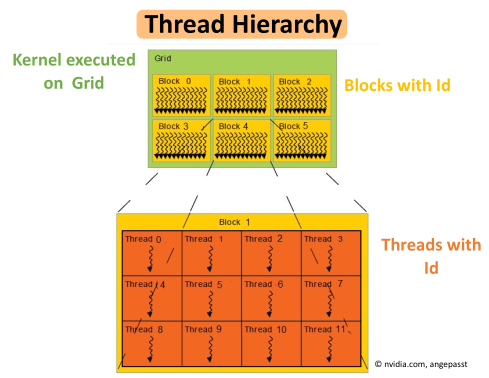
\includegraphics[width=.9\linewidth]{img/thread_hierarchy.png}
\end{center}
\captionof{figure}{Thread Hierarchy on GPU}\label{fig:thread-hierarchy-on-gpu}
}
\subparagraph{CUDA Memroy Model} \
\label{sec:org5b45a08}
All threads have access to the same global memory.
Each thread block has shared memory, which is visible to all threads of the block.
The shared memory is much faster because it is on-chip.
The variables in the kernel are normally stored in the regiester (fastest access).
Each thread has private local memory which resides in device memory (slow).
Only when all register are used the GPU uses the local memory.
\subparagraph{Memory Coalescing} \
\label{sec:org5ae39e7}
\lstset{language=C,label= ,caption= ,captionpos=b,numbers=none}
\begin{lstlisting}
data[(Expression without threadIdx.x) + threadIdx.x]
\end{lstlisting}

{
\begin{center}
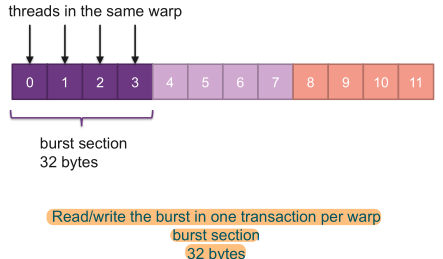
\includegraphics[width=.9\linewidth]{img/memory_coalescing.png}
\end{center}
\captionof{figure}{Memory Coalescing}\label{fig:memory-coalescing}
}

{
\begin{center}
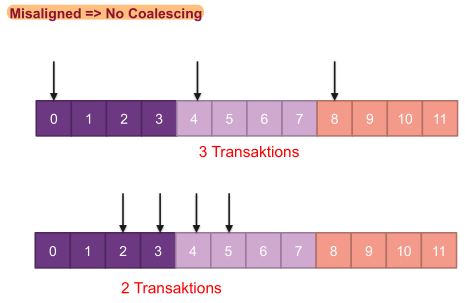
\includegraphics[width=.9\linewidth]{img/no_memory_coalescing.png}
\end{center}
\captionof{figure}{No Memory Coalescing}\label{fig:no-memory-coalescing}
}
\subparagraph{Branching / Divergenz} \
\label{sec:org46a0e38}
The Streaming Multiprocessor executes the instruction of one branch per warp.
All the other threads have to wait.
Then the next branch is executed.
Some threads have to wait again.
This leads to performance problem.
Single \texttt{if} is not a problem
\section{MPI}
\label{sec:orga09107b}
\subparagraph{Hybrid Memory Architecture} \
\label{sec:orgd054c8c}
Most modern supercomputers use a hybrid memory architecture.
All processors in a machine can share the memory (\href{../../../roam/20220524184828-uniform_memory_access.org}{UMA}).
The memory from a remote machine can be requested programmatically (\href{../../../roam/20220518180028-what_is_the_numa_model.org}{NUMA}).

{
\begin{center}
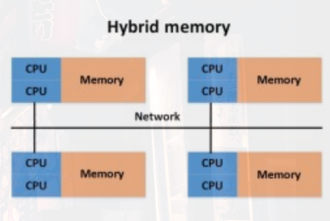
\includegraphics[width=.9\linewidth]{img/hybrid_memory_architecture.png}
\end{center}
\captionof{figure}{Hybrid Memory Architecture}\label{fig:hybrid-memory-architecture}
}
\subparagraph{SPMD / MPMD} \
\label{sec:org8a92af3}
{
\begin{center}
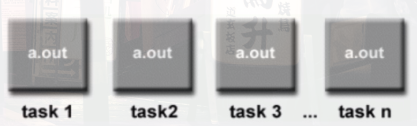
\includegraphics[width=.9\linewidth]{img/spmd_model.png}
\end{center}
\captionof{figure}{Single Program Multiple Data}\label{fig:spmd}
}

{
\begin{center}
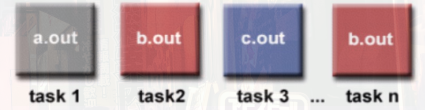
\includegraphics[width=.9\linewidth]{img/mpmd_model.png}
\end{center}
\captionof{figure}{Multiple Program Multiple Data}\label{fig:mpmd}
}
\subparagraph{Communication Modes} \
\label{sec:org5186ebf}
Scatter, Gather, Broadcast
\subparagraph{MPI Message} \
\label{sec:org50ad26e}
When one process transfers data to another process the following data are sent:
\begin{itemize}
\item ID of the sender
\item ID of the receiver
\item Data type to be sent (int, float, char, \ldots{})
\item number of data items
\item the data itself
\item a message type identifier
\end{itemize}
\subparagraph{Broadcast} \
\label{sec:orgdb6e4df}
The root note sends the data to all notes.
As soon as a node receives the data it sends the data to other notes.
Because of this, \texttt{MPI\_Bcast} is faster than \texttt{MPI\_Send}.
\subparagraph{Structure} \
\label{sec:org3d5809d}
\lstset{language=C,label= ,caption= ,captionpos=b,numbers=none}
\begin{lstlisting}
int main(int argc, char* argv[]) {
  MPI_Init(&argc, &argv);
  int rank;
  int size;
  MPI_Comm_rank(MPI_COMM_WORLD, &rank);
  MPI_Comm_size(MPI_COMM_WORLD, &size);

  if (rank == ROOT_RANK) {
    MPI_Gather(/**/);
  } else {
    MPI_Gather(/**/);
  }
  MPI_Finalize();
  return 0;
}
\end{lstlisting}
\subparagraph{OpenMP} \
\label{sec:org21a8486}
OpenMP is an API for writing multithreaded code in \href{../../../roam/20211008113512-c.org}{C}, \href{../../../roam/20210920103243-c.org}{CPP}.
OpenMP uses \texttt{\#pragma} to insert instructions.

\lstset{language=C,label= ,caption= ,captionpos=b,numbers=none}
\begin{lstlisting}
#include <stdio.h>
#include <omp.h>

int main(void)
{
#pragma omp parallel
  printf("Hello, world.\n");
  return 0;
}
\end{lstlisting}
\section{Laws}
\label{sec:org172dc90}
\subparagraph{Amdahls's law} \
\label{sec:orga3acba2}
\begin{equation}
  \text{SpeedUp} = \frac{1}{s + \frac{p}{N}}
\end{equation}

\subparagraph{Gutafson's law} \
\label{sec:org8363707}
\begin{description}
\item[{s}] serial part
\item[{p}] parallel part
\item[{N}] number of processes
\end{description}
\begin{equation}
\text{SpeedUp} = s + p \cdot N = s + (1-s) \cdot N
\end{equation}


\end{multicols}
\end{document}